\section{Nurul Izza Hamka - 1174062}
\subsection{Teori}
\begin{enumerate}

\item Jelaskan dengan ilustrasi gambar sendiri apa perbedaan antara vanilla GAN dan cGAN.

Vanilla GAN biasanya tidak memiliki jaringan saraf convolutional (CNN) di jaringan mereka. Ini diusulkan untuk pertama kalinya dengan diperkenalkannya DCGAN. Dalam vanilla GANs, tidak ada kontrol atas kategori gambar yang dihasilkan. Vanilla GAN hanya dapat mempelajari satu kategori dan sangat sulit untuk merancang GAN untuk beberapa kategori.\\
Sedangkan Conditional GANs (cGANs) adalah perpanjangan dari model GAN. Mereka memungkinkan untuk generasi gambar yang memiliki kondisi atau atribut tertentu dan telah terbukti lebih baik daripada vanilla GAN sebagai hasilnya. cGANs memperluas gagasan vanilla GAN dan memungkinkan kami untuk mengontrol output dari jaringan generator.

\begin{figure}
	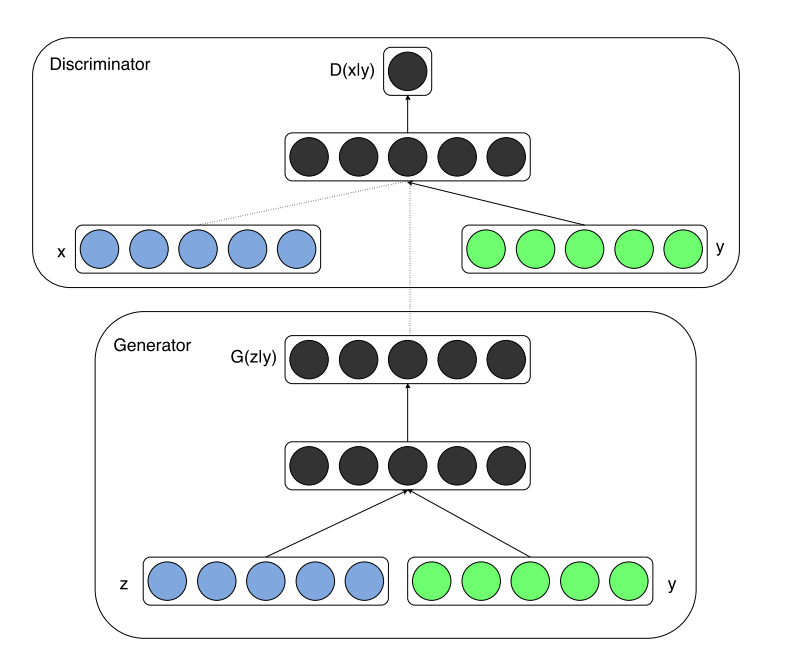
\includegraphics[width=4cm]{figures/1174062/9/nomor1.png}
	\centering
	\caption{Ilustrasi Nomor 1 }
\end{figure}

\item Jelaskan dengan ilustrasi gambar sendiri arsitektur dari Age-cGAN.

Age-cGan terdiri dari empat jaringan: encoder, FaceNet, jaringan generator, dan jaringan diskriminator. Dengan encoder, kita belajar pemetaan terbalik dari gambar wajah input dan kondisi usia dengan vektor laten. FaceNet adalah jaringan pengenalan wajah yang mempelajari perbedaan antara gambar input x dan gambar yang direkonstruksi. 

\begin{figure}
	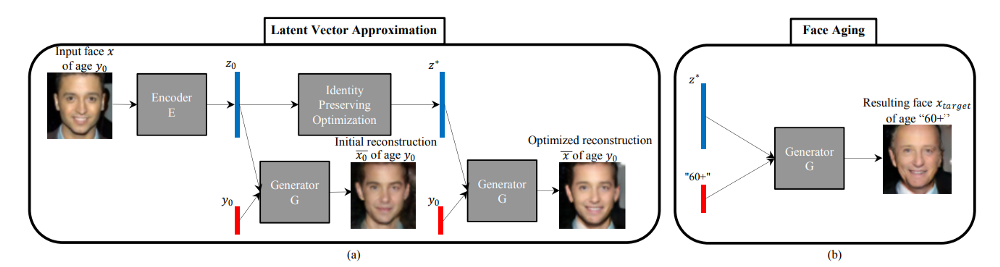
\includegraphics[width=4cm]{figures/1174062/9/nomor2.png}
	\centering
	\caption{Ilustrasi Nomor 2 }
\end{figure}

\item Jelaskan dengan ilustrasi gambar sendiri arsitektur encoder network dari Age-Cgan.

Jaringan encoder adalah jaringan saraf convolutional yang mendalam. Tujuan utama dari jaringan encoder adalah untuk mengasilkan sebuah vector laten dari gambar yang telah digunakan. Pada dasarnya, ini mengambil gambar dari dimensi (64, 64, 3) dan mengubahnya menjadi vektor 100 dimensi.

\item Jelaskan dengan ilustrasi gambar sendiri arsitektur generator network dari Age-cGAN.

A Generator Network: Dibutuhkan representasi tersembunyi dari gambar wajah dan vektor kondisi sebagai input dan menghasilkan gambar.\\
Jaringan Generator adalah CNN dan dibutuhkan vektor laten 100 dimensi dan vektor kondisi y, dan mencoba menghasilkan gambar realistis dari dimensi (64, 64, 3)

\item Jelaskan dengan ilustrasi gambar sendiri arsitektur discriminator network dari Age-cGAN.

Jaringan Diskriminator, mencoba membedakan antara gambar asli dan gambar palsu.

\item Jelaskan dengan ilustrasi gambar sendiri apa itu pretrained Inception-ResNet-2-Model.

Inception-ResNet-v2 adalah jaringan saraf convolutional yang dilatih pada lebih dari satu juta gambar dari database ImageNet. Jaringannya memiliki 164 lapisan dan dapat mengklasifikasikan gambar ke dalam 1000 kategori objek, seperti keyboard, mouse, pensil, dan banyak binatang. 

\begin{figure}
	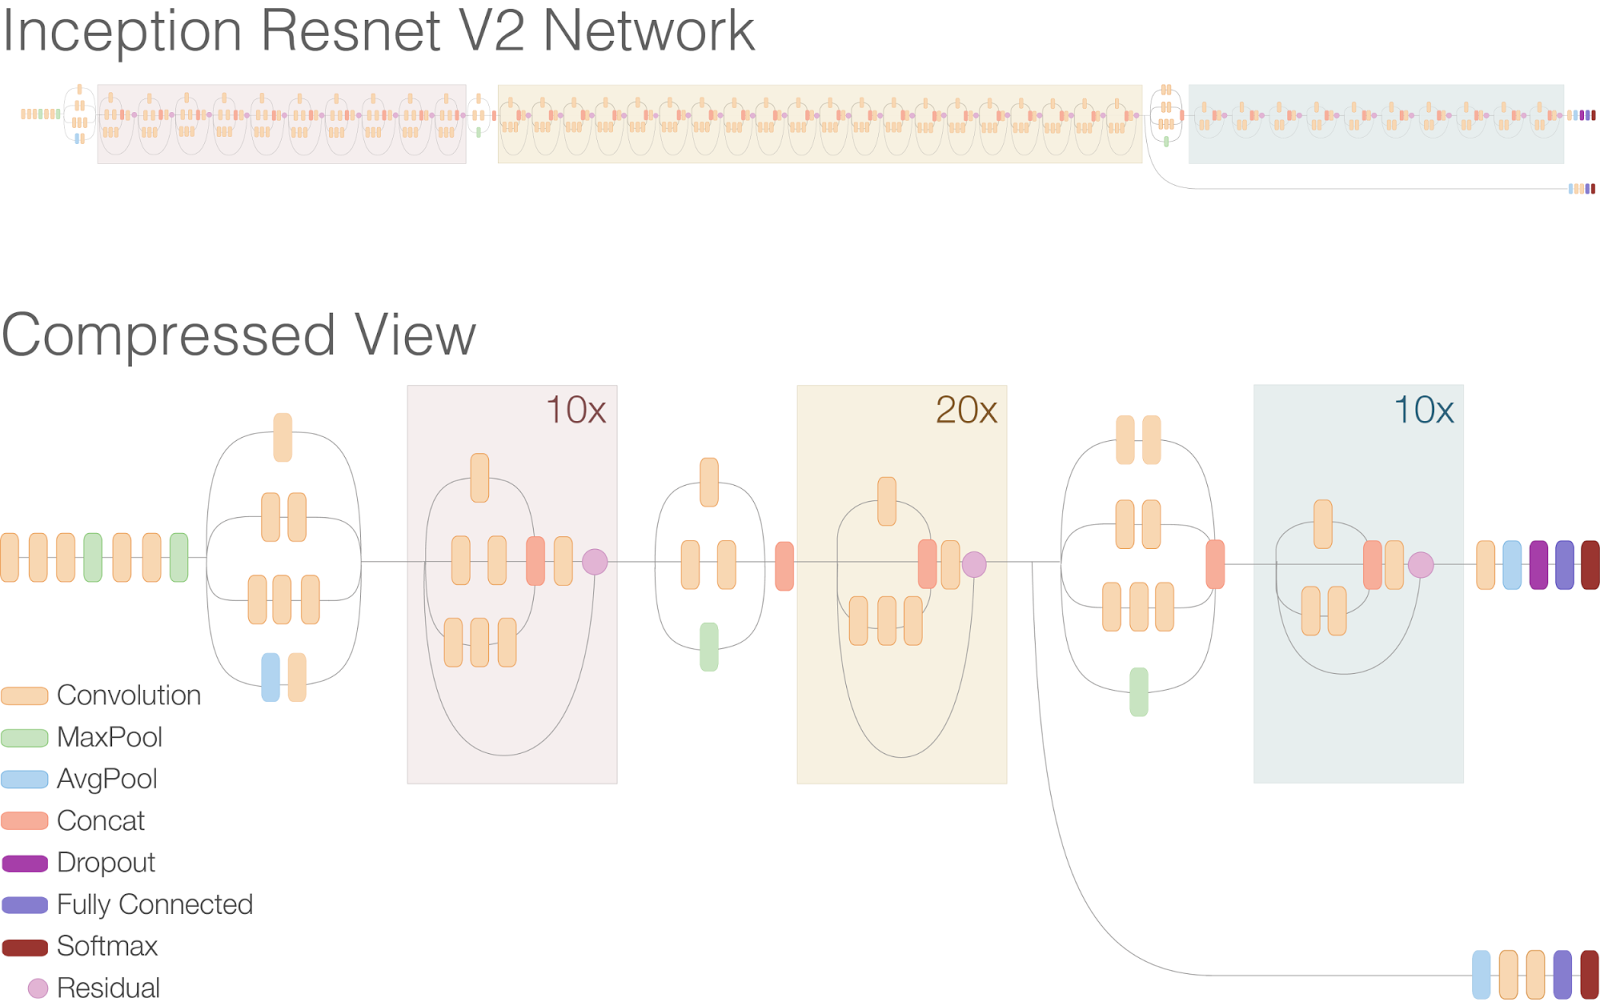
\includegraphics[width=4cm]{figures/1174062/9/nomor6.png}
	\centering
	\caption{Ilustrasi Nomor 6 }
\end{figure}

\item Jelaskan dengan ilustrasi gambar sendiri arsitektur Face reconition network Age-cGAN. 

Tujuan utama dari Face reconition adalah untuk mengenali identitas seseorang dalam gambar yang diberikan.

\begin{figure}
	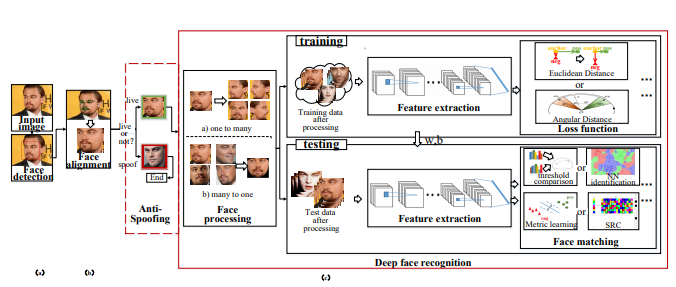
\includegraphics[width=4cm]{figures/1174062/9/nomor7.png}
	\centering
	\caption{Ilustrasi Nomor 7 }
\end{figure}

\item Sebutkan dan jelaskan disertai contoh-contoh tahapan dari Age-cGAN.  
a. Conditional GAN training, Pada tahap ini adalah melatih generator jaringan dan jaringan diskriminator. Setelah dilatih, jaringan generator dapat menghasilkan gambar wajah yang buram.\\
b. Initial latent vector approximation, Pada tahap ini adalah melatih jaringan encoder. Setelah dilatih, jaringan encoder akan mulai menghasilkan vektor laten dari distribusi yang dipelajari. Fungsi tujuan pelatihan untuk melatih jaringan encoder adalah kehilangan jarak Euclidean.\\
c. Latent vector optimization, Pada tahap ini adalah mengoptimalkan encoder dan jaringan generator.

\item Berikan contoh perhitungan fungsi training objektif.

\begin{figure}
	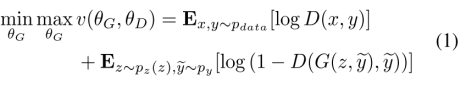
\includegraphics[width=4cm]{figures/1174062/9/nomor9.png}
	\centering
	\caption{Perhitungan Fungsi Training Objektif}
\end{figure}

Dimana:\\
-	log D (x, y) adalah kerugian untuk model Diskriminator.\\
-	log (1-D (G (x, y’), y’)) adalah kerugian untuk model Generator.\\
-	P (data) adalah distribusi dari semua gambar yang mungkin.\\

\item Berikan contoh dengan ilustrsi penjelasan dari Initial latent vector approximation.
-	Metode perkiraan awal vektor laten digunakan untuk memperkirakan vektor laten untuk mengoptimalkan rekonstruksi gambar wajah.\\
-	Encoder adalah jaringan saraf yang mendekati vektor laten.\\
-	Kami melatih jaringan encoder pada gambar yang dihasilkan dan gambar nyata.\\
-	Setelah dilatih, jaringan encoder akan mulai menghasilkan vektor laten dari distribusi yang dipelajari.\\
-	Fungsi tujuan pelatihan untuk melatih jaringan encoder adalah kehilangan jarak Euclidean\\

\item Berikan contoh peritungang latent vector optimazation.

\begin{figure}
	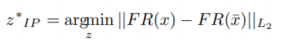
\includegraphics[width=4cm]{figures/1174062/9/nomor11.png}
	\centering
	\caption{Peritungang Latent Vector Optimazation}
\end{figure}


Dimana:\\
FR adalah jaringan pengenalan wajah. Persamaan ini menunjukkan bahwa jarak Euclidean antara gambar asli dan gambar yang direkonstruksi harus minimal. Pada tahap ini, kami mencoba meminimalkan jarak untuk memaksimalkan pelestarian identitas.
\end{enumerate}

\subsection{Praktek Program}
\begin{enumerate}

\item Jelaskan bagaimana cara extract file dari Age-cGAN menggunakan goole colab.

	\hfill\break
	\lstinputlisting[firstline=8, lastline=12]{src/1174062/9/1174062.py}
	
Kode diatas adala untuk melakukan ekstrak file menggunakan google colab.

\item Jelaskan bagaimana kode program bekerja untuk melakukan load terhadap dataset yang suda di ekstrak, termaksud bagaimana penjelasan kode program perhitungan usia.

	\hfill\break
	\lstinputlisting[firstline=13, lastline=38]{src/1174062/9/1174062.py}
	
Pertama Load file wiki.mat\\
kedua  load semua file\\
ketiga Daftar nomor tanggal seri Matlab\\
keempat Daftar tahun ketika foto diambil\\
kelima Hitung usia untuk semua dobs\\
selanjutnya Buat daftar tupel yang berisi sepasang jalur dan usia gambar
Terakhir Kembalikan daftar semua gambar dan usia masing-masing
	
\item Jelaskan bagaimana kode program The Encoder Network bekerja dijelaskan dengan bahawa awam dengan ilustrasi sederhana.

	\hfill\break
	\lstinputlisting[firstline=34, lastline=72]{src/1174062/9/1174062.py}
	
\item Jelaskan bagaimana kode program The Generator Network bekerja dijelaskan dengan bahawa awam dengan ilustrasi sederhana.

	\hfill\break
	\lstinputlisting[firstline=74, lastline=113]{src/1174062/9/1174062.py} 
	
\item Jelaskan bagaimana kode program The Discriminator Network bekerja dijelaskan dengan bahawa awam dengan ilustrasi sederhana.

	\hfill\break
	\lstinputlisting[firstline=115, lastline=147]{src/1174062/9/1174062.py}
	
\item Jelaskan bagaimana kode program Training cGAN bekerja dijelaskan dengan bahawa awam dengan ilustrasi sederhana.

	\hfill\break
	\lstinputlisting[firstline=149, lastline=166]{src/1174062/9/1174062.py} 
	
\item Jelaskan bagaimana kode program Initial dan latent vector approximation bekerja dijelaskan dengan bahawa awam dengan ilustrasi sederhana.

	\hfill\break
	\lstinputlisting[firstline=168, lastline=216]{src/1174062/9/1174062.py} 

\end{enumerate}

\subsection{Bukti Tidak Plagiat}
\begin{figure}
	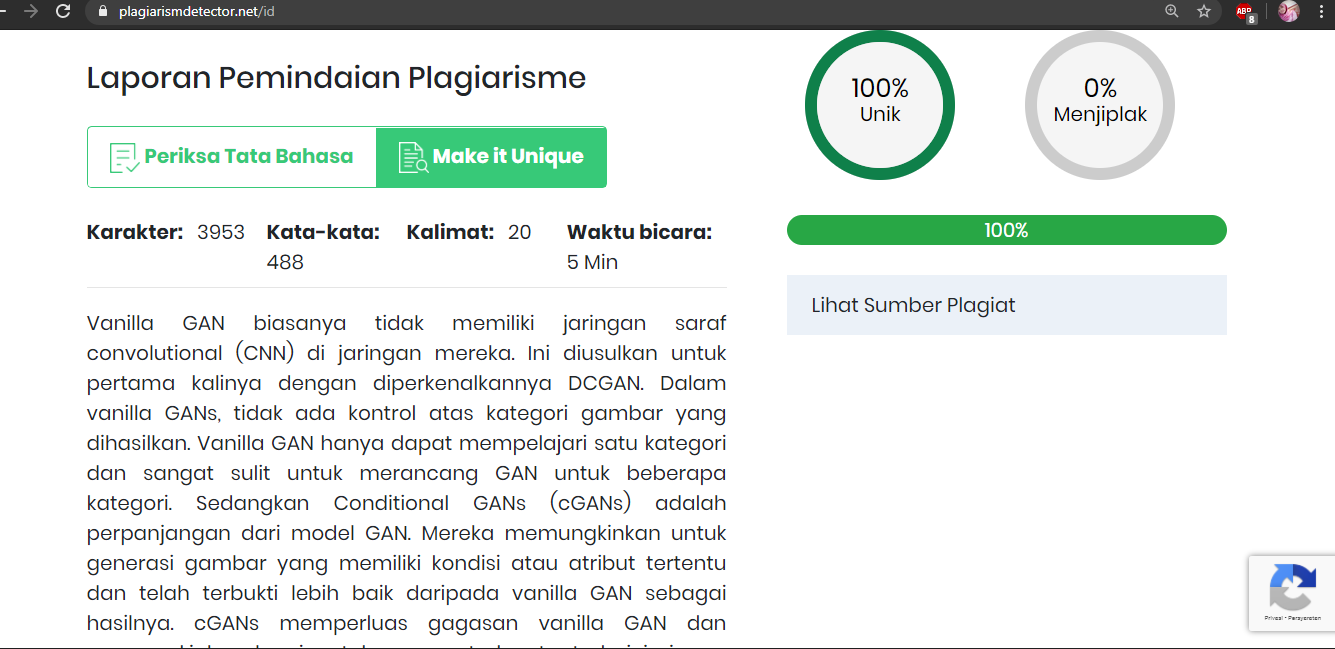
\includegraphics[width=4cm]{figures/1174062/9/buktiplagiat.png}
	\centering
	\caption{Hasil Tidak Plagiat}
\end{figure}

\subsection{Link Youtube}
\href{https://www.youtube.com/watch?v=GV18e_jp6DE}{Chapter9}. 